\documentclass[preview]{standalone}

\usepackage{amsmath}
\usepackage{amssymb}
\usepackage{tikz}
\usetikzlibrary{decorations.pathreplacing}
\usepackage{stellar}
\usepackage{definitions}

\begin{document}

\id{module-socle-cyclic-primary-components}
\genpage

\section{Generators of the socle}

\begin{snippetproposition}{primary-socle-generators}{Generators and independence in the socle}
    Let \(A\) be a \principalidealdomain, let \(p\in A\) be a
    \primeelement, and put \(K=A/(p)\). A finite \set
    \[
        \mathcal X=\{v_1,\ldots,v_r\}
        \subseteq\modulesocle_p(M)
    \]
    generates \(\modulesocle_p(M)\) as an \(A\)-\module
    \ifandonlyif it spans it as a \(K\)-\vectorspace.

    Moreover, \(\mathcal X\) is linearly independent over \(K\)
    \ifandonlyif every relation
    \[
        a_1v_1+\cdots+a_rv_r=0_M,
        \qquad a_i\in A,
    \]
    has \(a_i\in(p)\) for every \(i\).
\end{snippetproposition}

\begin{snippetproof}{primary-socle-generators-proof}{primary-socle-generators}{Generators and independence in the socle}
    If \(w=\sum_i a_iv_i\) with \(a_i\in A\), then
    \[
        w=\sum_i(a_i+(p))v_i
    \]
    as a linear combination over \(K\). Conversely, every \(K\)-linear
    combination can be written using representatives in \(A\).

    A relation over \(A\) induces
    \[
        \sum_i(a_i+(p))v_i=0_M
    \]
    over \(K\). Thus \(K\)-linear independence is equivalent to
    \(a_i+(p)=0\), or \(a_i\in(p)\), for every \(i\). Notice that
    nonzero elements of the socle are never \(A\)-linearly independent,
    because they are annihilated by the nonzero scalar \(p\).
\end{snippetproof}

\section{Cyclic primary modules}

\begin{snippetlemma}{cyclic-primary-module-socle}{Socle of a cyclic primary module}
    Let \(M=Av\) be a cyclic \(p\)-\primarymodule with
    \[
        \moduleann(v)=(p^n),
        \qquad n\geq1.
    \]
    Then
    \[
        \modulesocle_p(M)=A(p^{n-1}v)
        \moduleisomorphic (p^{n-1})/(p^n)
        \submoduleleq A/(p^n),
    \]
    and
    \[
        M/\modulesocle_p(M)\moduleisomorphic A/(p^{n-1}).
    \]
\end{snippetlemma}

\begin{snippetproof}{cyclic-primary-module-socle-proof}{cyclic-primary-module-socle}{Socle of a cyclic primary module}
    The first isomorphism theorem gives \(M\moduleisomorphic A/(p^n)\),
    with \(v\) corresponding to \(1+(p^n)\). In this quotient,
    \begin{align*}
        \modulesocle_p(A/(p^n))
        &=
        \{a+(p^n)\suchthat pa\in(p^n)\}\\
        &=
        \{a+(p^n)\suchthat p^n\divides pa\}.
    \end{align*}
    Since \(A\) is an \integraldomain,
    \[
        p^n\divides pa
        \ifandonlyif
        p^{n-1}\divides a.
    \]
    Hence
    \[
        \modulesocle_p(A/(p^n))=(p^{n-1})/(p^n),
    \]
    which corresponds to \(A(p^{n-1}v)\) in \(M\). The third
    isomorphism theorem yields
    \[
        \frac{A/(p^n)}{(p^{n-1})/(p^n)}
        \moduleisomorphic A/(p^{n-1}).
    \]
\end{snippetproof}

\begin{snippetnote}{cyclic-primary-module-socle-n-one}{The case \(n=1\)}
    If \(n=1\), then
    \[
        M\moduleisomorphic A/(p),
        \qquad
        \modulesocle_p(M)=M.
    \]
    The quotient by the socle is the zero module, consistently with
    \(A/(p^0)=A/(1)=0\).
\end{snippetnote}

\section{Recovering the cyclic summands}

\begin{snippetproposition}{primary-cyclic-exponents-uniqueness}{Uniqueness of the primary exponents}
    Suppose that the finitely generated \(p\)-\primarymodule \(M\) has a
    decomposition
    \[
        M\moduleisomorphic
        \bigoplus_{i=1}^{r}A/(p^{n_i}),
        \qquad
        1\leq n_1\leq\cdots\leq n_r.
    \]
    Then \(r\) and the multiset \(\{n_1,\ldots,n_r\}\) are determined by
    \(M\).
\end{snippetproposition}

\begin{snippetproof}{primary-cyclic-exponents-uniqueness-proof}{primary-cyclic-exponents-uniqueness}{Uniqueness of the primary exponents}
    Define intrinsically
    \[
        M_1=M,
        \qquad
        M_{h+1}=M_h/\modulesocle_p(M_h).
    \]
    Repeated use of the cyclic-socle lemma gives
    \[
        M_h\moduleisomorphic
        \bigoplus_{\substack{1\leq i\leq r\\n_i\geq h}}
        A/(p^{n_i-h+1}).
    \]
    Therefore
    \[
        \dim_{A/(p)}\modulesocle_p(M_h)
        =
        \#\{i\suchthat n_i\geq h\}.
    \]
    In particular,
    \[
        r=\dim_{A/(p)}\modulesocle_p(M_1),
    \]
    and the number of exponents equal to \(h\) is
    \[
        \dim\modulesocle_p(M_h)
        -
        \dim\modulesocle_p(M_{h+1}).
    \]
    These dimensions depend only on \(M\), so the exponents are unique.
\end{snippetproof}

\begin{snippet}{primary-cyclic-columns-visualization}
    Represent each summand \(A/(p^{n_i})\) by a column of height \(n_i\).
    The socle is the bottom row, and quotienting by it removes that row.
    \[
        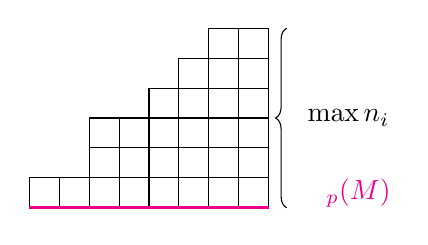
\begin{tikzpicture}[scale=0.38]
            \foreach \x/\h in {0/1,1/1,2/3,3/3,4/4,5/5,6/6,7/6} {
                \foreach \y in {1,...,\h} {
                    \draw (\x,\y-1) rectangle (\x+1,\y);
                }
            }
            \draw[very thick, magenta] (0,0) -- (8,0);
            \node[magenta] at (11,0.5) {\(\modulesocle_p(M)\)};
            \draw[decorate, decoration={brace, amplitude=4pt}]
                (8.6,0) -- (8.6,6)
                node[midway, right=4pt] {\(\max n_i\)};
        \end{tikzpicture}
    \]
    After quotienting by the socle, the surviving columns are one unit
    shorter:
    \[
        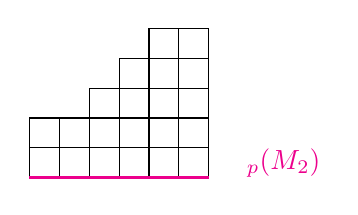
\begin{tikzpicture}[scale=0.38]
            \foreach \x/\h in {2/2,3/2,4/3,5/4,6/5,7/5} {
                \foreach \y in {1,...,\h} {
                    \draw (\x,\y-1) rectangle (\x+1,\y);
                }
            }
            \draw[very thick, magenta] (2,0) -- (8,0);
            \node[magenta] at (10.5,0.5) {\(\modulesocle_p(M_2)\)};
        \end{tikzpicture}
    \]
    Iterating reveals all column heights, hence all exponents \(n_i\).
\end{snippet}

\end{document}
